\documentclass{article}
\usepackage[utf8]{inputenc}
\usepackage[margins=0.5in]{geometry}
\usepackage{wrapfig}
\usepackage{graphicx}
\usepackage{enumitem}

\renewcommand{\v}[1]{\textbf{#1}}
\newcommand{\ddt}[1]{\frac{d{#1}}{dt}}

\begin{document}
\begin{center}
\textbf{ \large MEGN 505 Advanced Dynamics\\ 
Fall 2025 \\
Midterm Exam 1} \\
\today
\end{center}

For this midterm exam, you will have 48 hours to work through the two problems in the document and put together your solutions and answers to the questions. You may use any of the class resources in working through these problems, but do not search for any specifics of any problems online. I expect this exam to represent your own work, so do not work with any of your peers.
\\

% \begin{wrapfigure}{r}{2.5in}
% \vspace{-20pt}
% \begin{center}
% \includegraphics[width=2.5in]{Cart.png}
% \end{center}
% \vspace{-20pt}
% \end{wrapfigure}


% Greenwood 1.14

\begin{wrapfigure}{r}{2in}
\vspace{-20pt}
\begin{center}
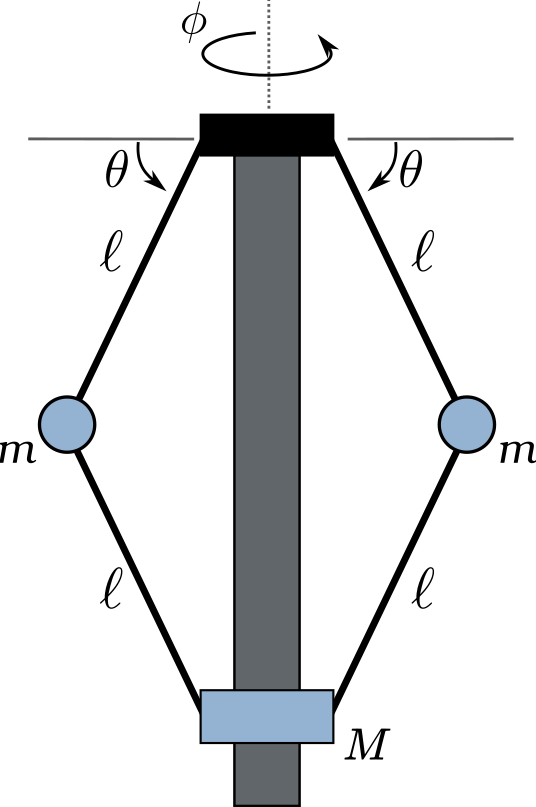
\includegraphics[width=2in]{FlyBall.png}
\end{center}
\vspace{-20pt}
\end{wrapfigure}


\noindent \textbf{Problem 1}: A flyball governor is constructed of 2 balls of mass \(m\) located at the end of a massless bar of length \(\ell\), each of which is attached to a freely-sliding collar of mass \(M\) by another massless bar of length \(\ell\). Define the angle of the top bar down from the horizontal as \(\theta\) and the rotation of the entire assembly around the vertical axis as the angle \(\phi\). \\

\noindent (a) Use the vector differentiation formula to write the velocity of each particle. \\

\noindent (b) What is the minimal set of generalized coordinates of the system? What is a redundant set that you could consider? \\

\noindent (c) Using the minimal set of coordinates, calculate the generalized velocity, \(\vec{\gamma}_ij\) for that generalized coordinates as if you were solving this problem with D'Alembert's Principle (but don't work through the entire solution). \\

\noindent (d) Construct the Lagrangian and derive the equations of motion for each generalized coordinate \(q_i\) of the system. \\

\noindent (e) Construct the Hamiltonian of the system and write the Hamiltonian equations of motion for each generalized coordinate \(q_i\) and its conjugate momentum \(p_i\). \\

\noindent (f) Are there any constants of motion for this problem? List them. \\

\noindent (g) Choose your own parameters and initial conditions for the problem. Using an initial value solver, numerically integrate Hamilton's equations of motion, and plot each \(q_i,p_i\) vs time. Additionally, plot \(\theta\) vs. \(\dot{\phi}\). \\

\noindent (h) If you wanted to solve for the forces in each bar to make sure that your string was strong enough, how could you solve for that? \\

\noindent (i) Discuss some possible approaches to the problem, including the Newtonian approach, which I didn't ask you to use here. Which approaches do you prefer? What are the different insights gained from each one? \\

\hline \vspace{10pt}

\clearpage
\begin{wrapfigure}{r}{2.5in}
    \vspace{-10pt}
    \begin{center}
        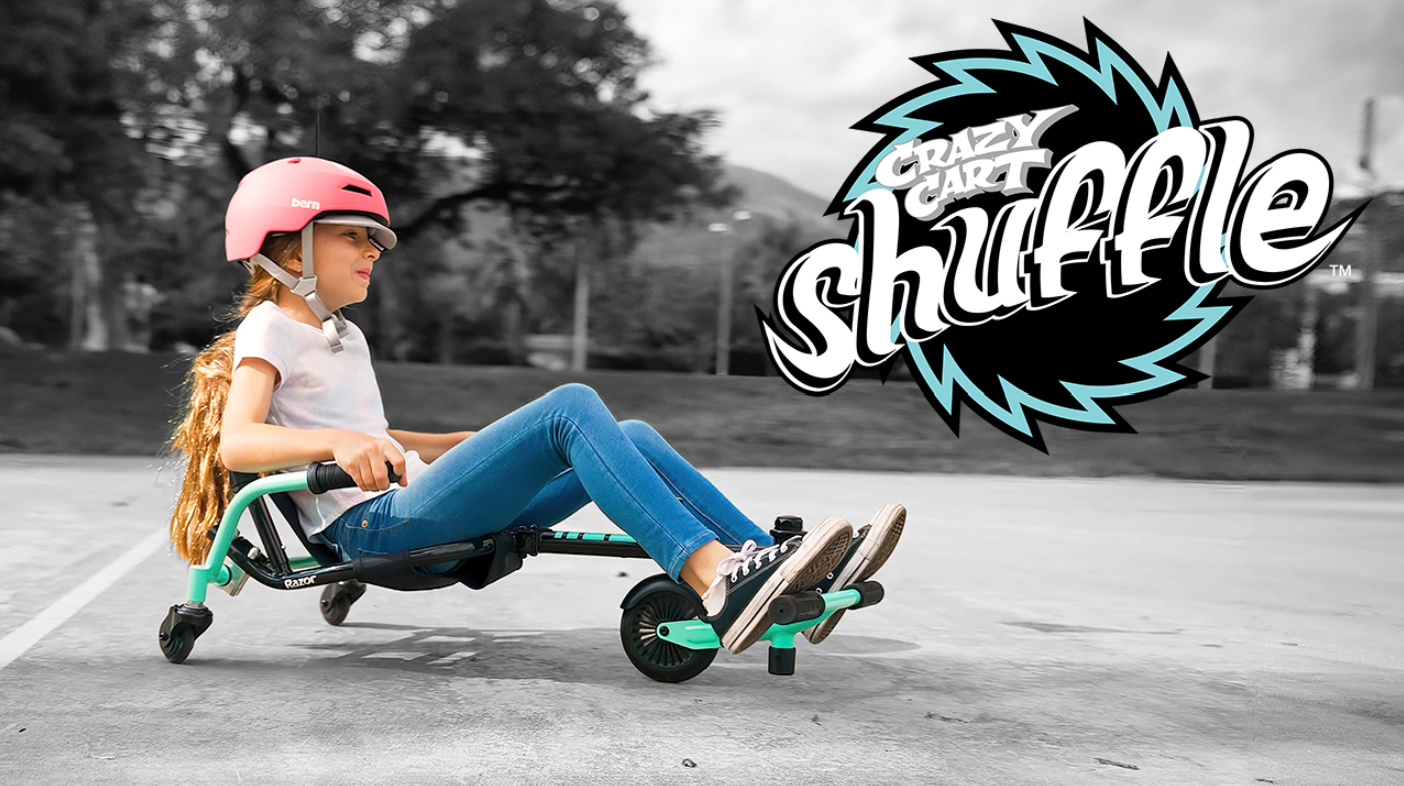
\includegraphics[width=2.5in]{CrazyCartShuffleWithRider.png}
        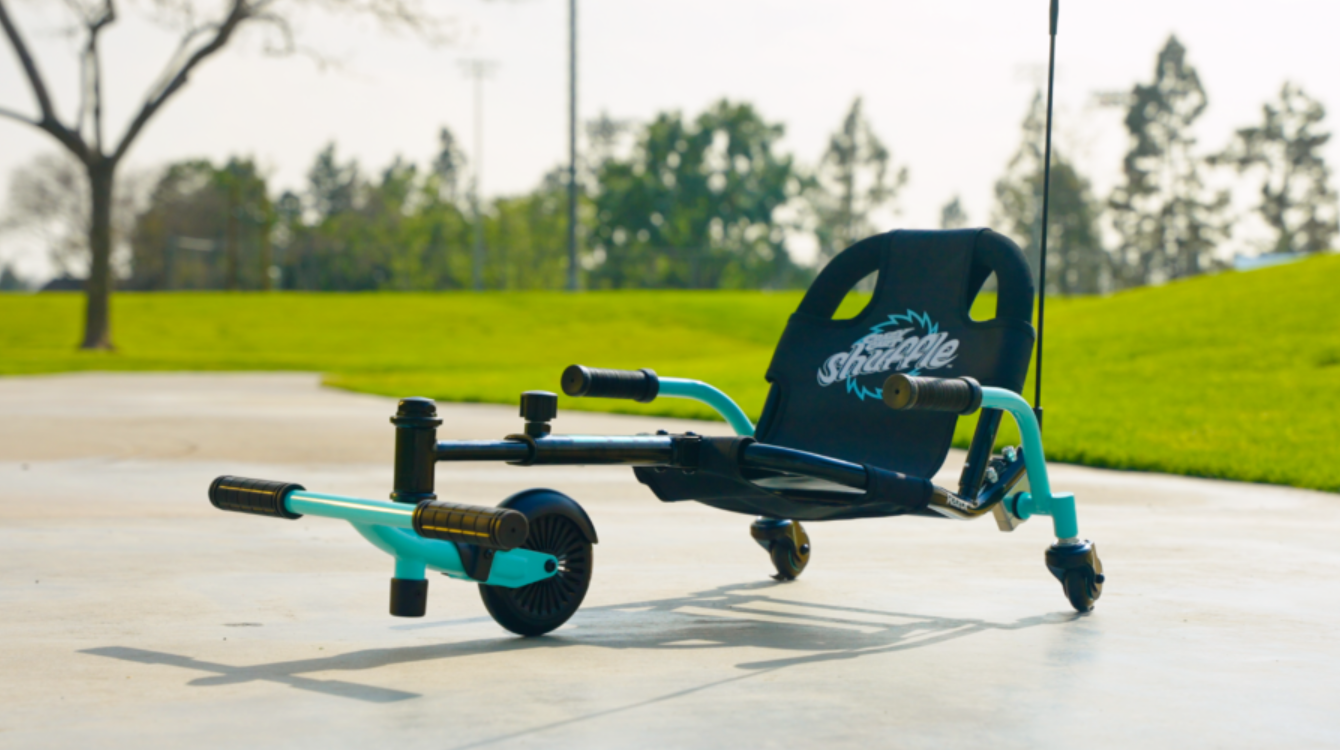
\includegraphics[width=2.5in]{CrazyCartShuffle.png}
        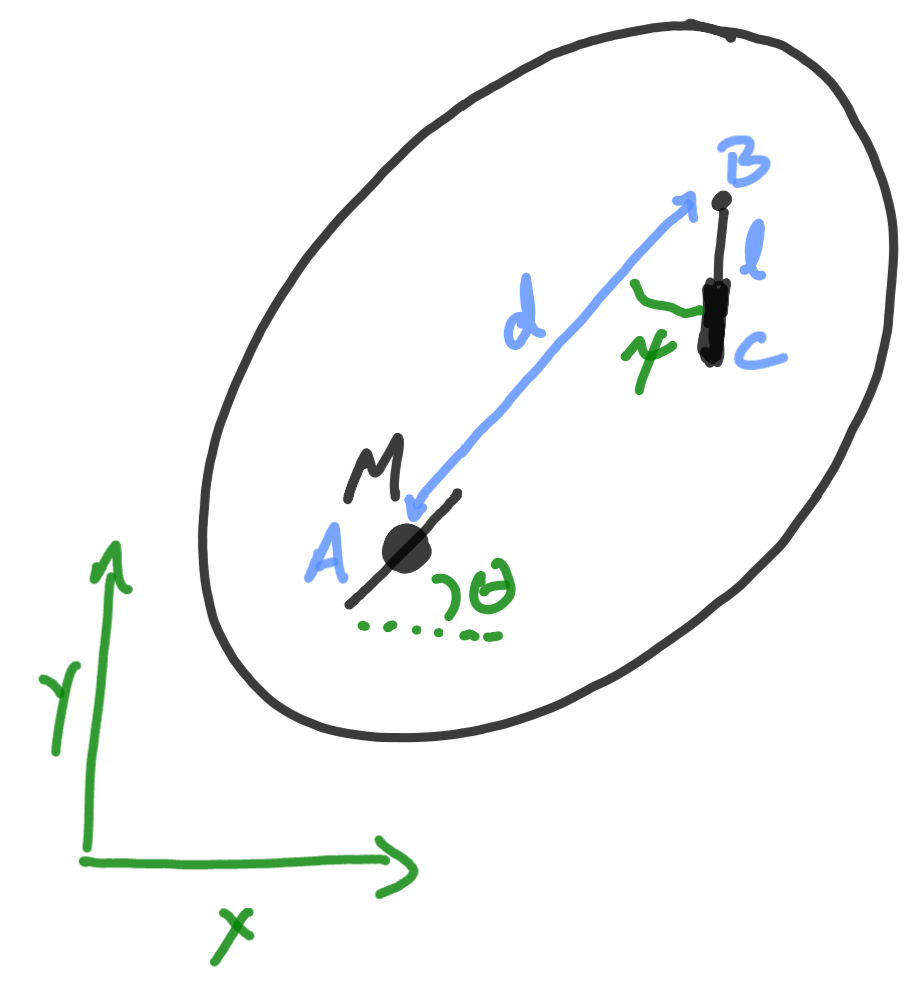
\includegraphics[width=2.5in]{CrazyCartModel.png}
    \end{center}
    \vspace{-50pt}
\end{wrapfigure}

\noindent \textbf{Problem 2}: For your second problem, consider the motion of the Razer Crazy Cart Shuffle. Kids make the Crazy Cart go by moving the bar on the front back and forth with their feet, meaning that it works entirely through nonholonomic constraints.

The center of mass is centered on the knife-edge constraint at \(A\), and its location in an inertial frame is given by \(x, y\). \(\theta\) represents the heading of the cart and \(\psi\) represents the angle between the front wheel to the heading of the cart. A second knife-edge constraint is located on the wheel (point \(C\)) at a distance \(\ell\) behind the pivot point \(B\). The pivot point \(B\) is located directly in line with the point \(A\) a distance \(d\) ahead. Treat the front wheel as massless.

\begin{enumerate}[label=\alph*.]
\item Write the two equations of constraint for the knife-edge constraints at \(A\) (\(\phi_1(q, \dot{q})=0\)) and \(C\) (\(\phi_2(q, \dot{q})=0\)). \textit{Hint: you may be able to use \(\phi_1\) to eliminate some terms from \(\phi_2\)}.

\item Use Lagrange's equations to derive the equations of motion for the cart in terms of Lagrange multipliers \(\lambda_1\) and \(\lambda_2\) corresponding to the two constraints.

\item Solve for \(\lambda_1\) and \(\lambda_2\).

\item Assume the rider rotates the front wheel back and forth with \(\psi=\frac{\pi}{6}\cos(\omega_0t)\) rad. Plot a trajectory of \(x\) vs \(y\) (the motion of the center of mass) as well as \(\theta\) vs \(t\), given that the Crazy Cart starts at rest with \(\theta_0=0\). You may choose your own values for mass, lengths, and moment of inertia.

\item What are the key assumptions that we have made in deriving this system? What practicalities of real systems would violate these assumptions? What effect do you expect that would have on the dynamics?
\end{enumerate}

\hline \vspace{10pt}

\end{document}